\chapter{Montaje Filastruder}
\label{ane:filastruder}

El control de temperatura del filastruder se realiza mediante un regulador PID modelo Sestos D1S. Conectándole el termopar tipo J y el cartucho calefactor, es capaz de regular la temperatura que deseemos del dado, el único problema es que no dispone de comunicaciones industriales, y sólo se puede introducir la temperatura deseada mediante el display que incorpora.
   	\begin{figure}[H]
            \centering
            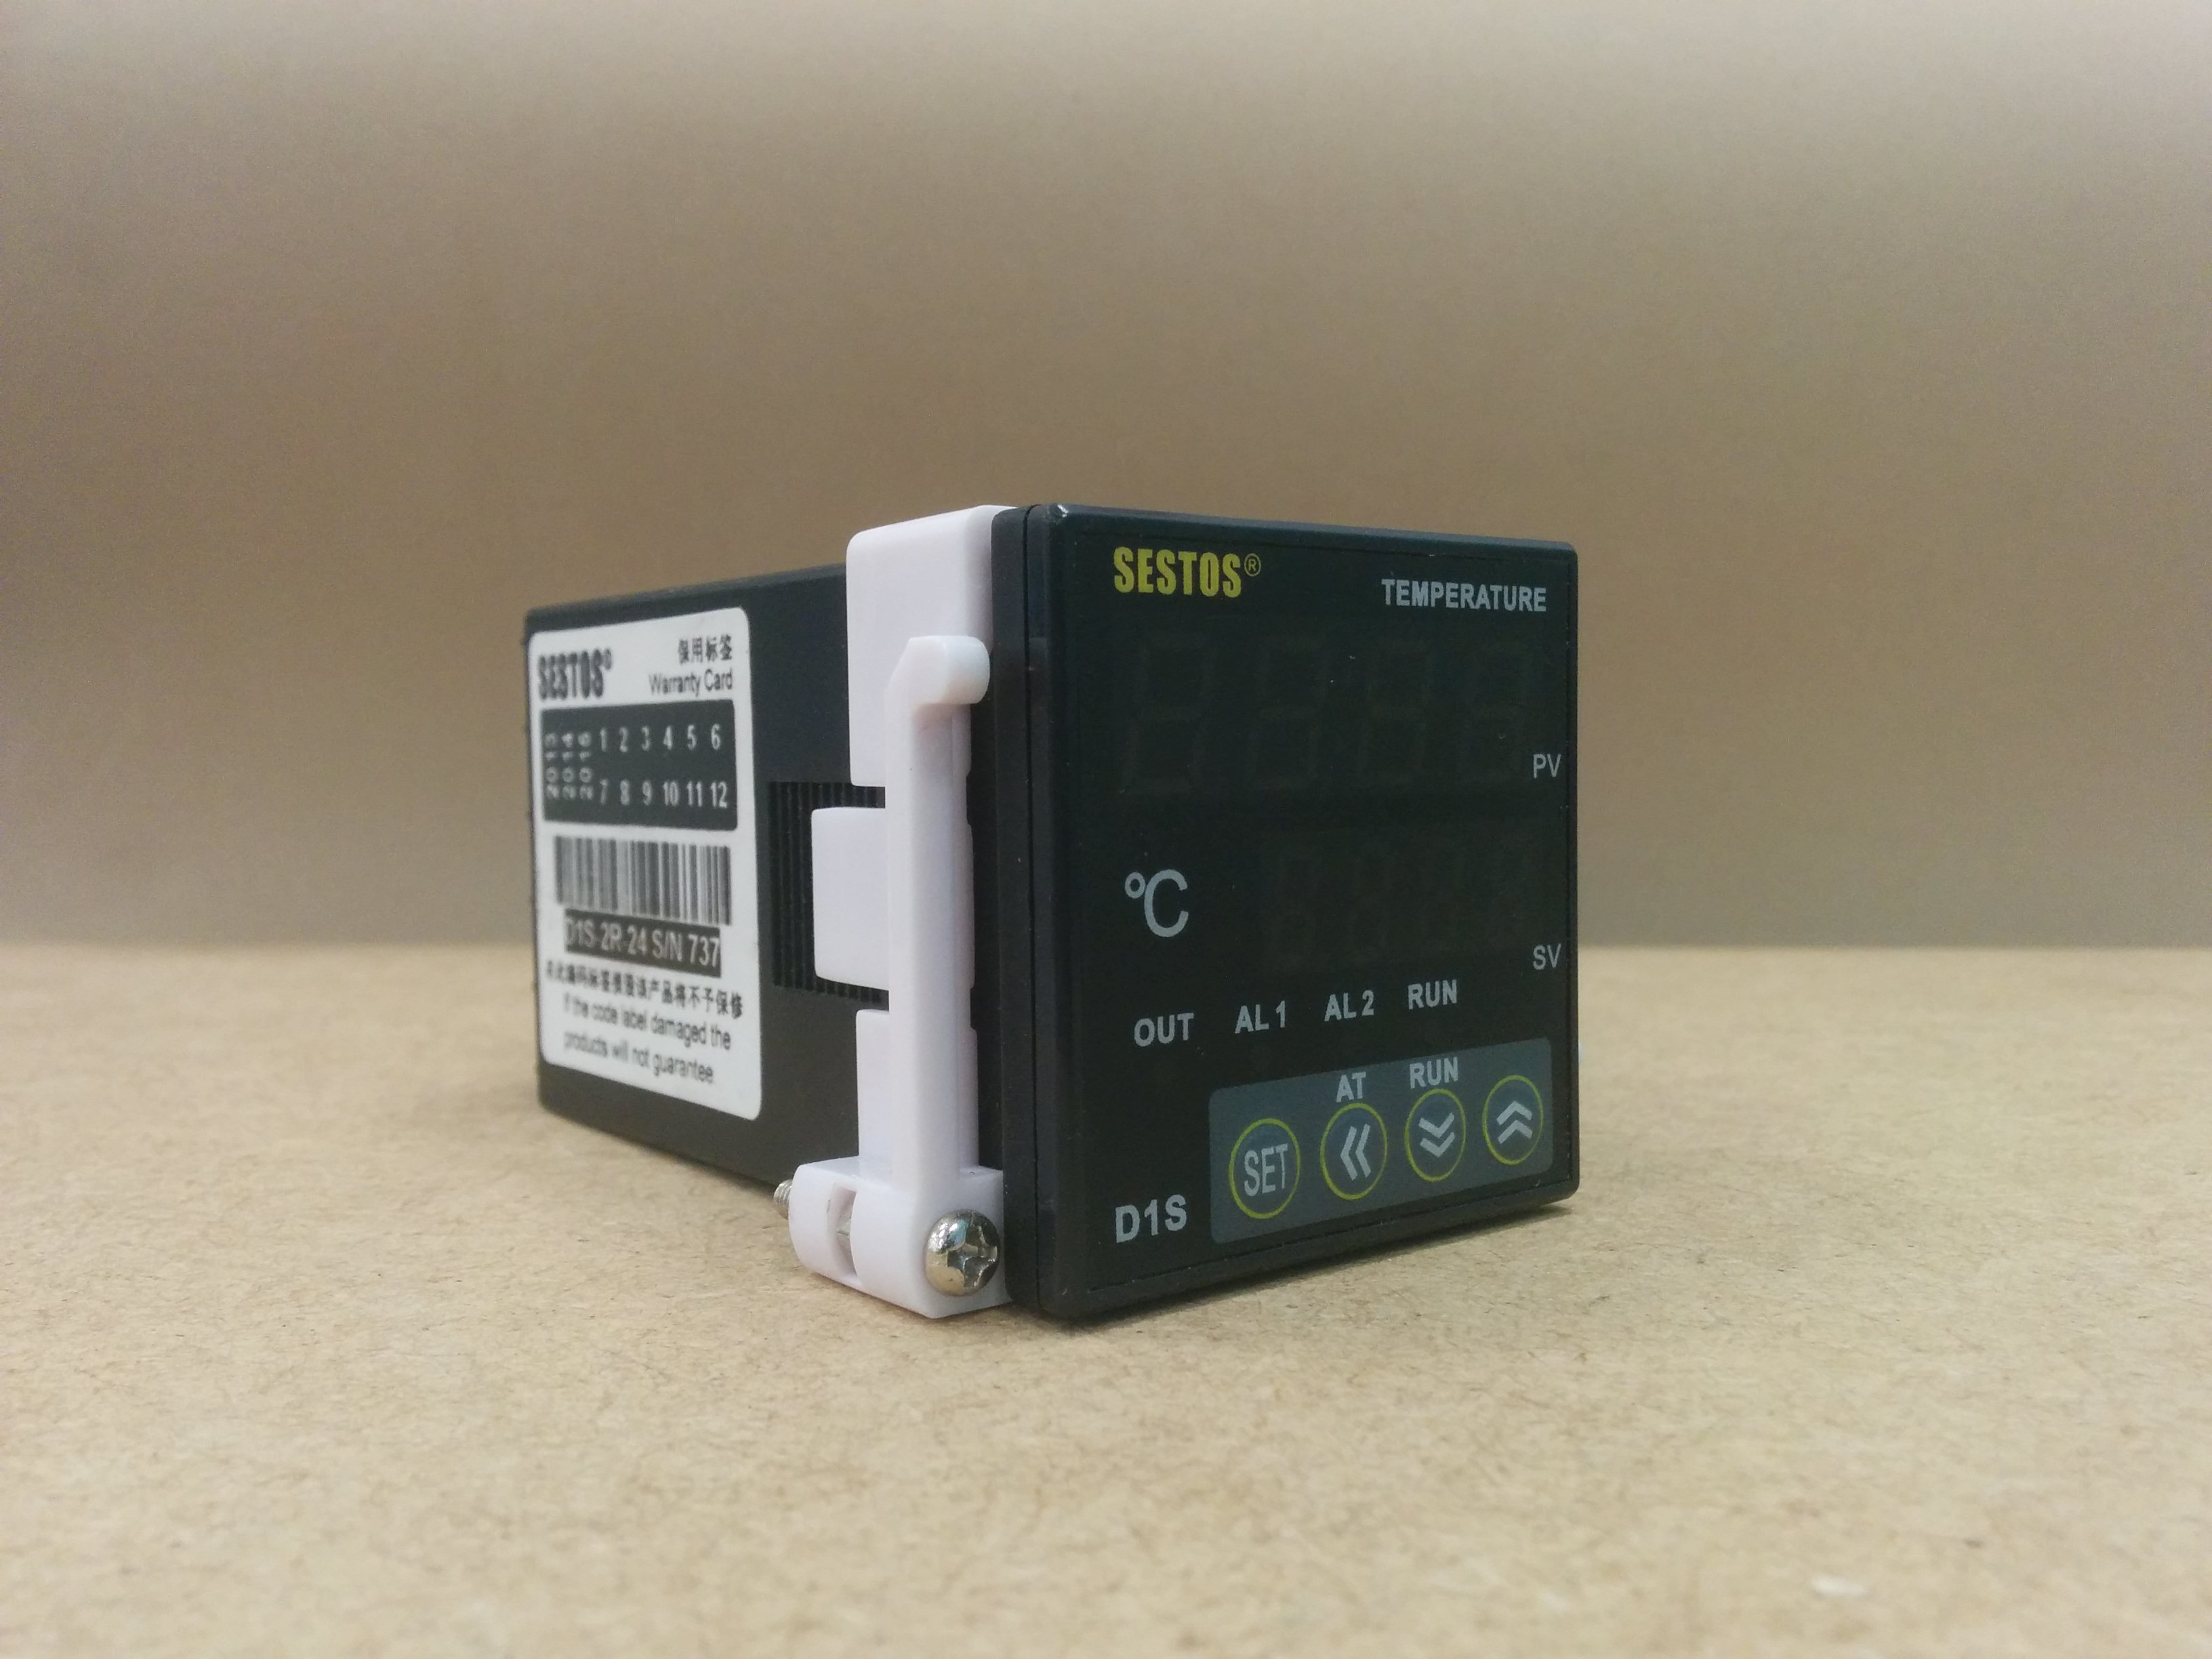
\includegraphics[width=0.6\textwidth]{images/filaextruder/IMG_20150814_123957.jpg}
            \caption{Controlador PID de temperatura Sestos}
            \label{fig:hardware_sestos}
    \end{figure}

Se decide entonces no usar el PID e integrar el control de temperatura en el PLC ya que, con el hardware que compramos tenemos dos entradas analógicas capaces de leer sensores de temperatura del tipo PT100. De este modo, podremos introducir dos zonas de calentamiento, una en el dado del cañón y otra en la entrada de los pellet para poder tener varios registros de temperaturas como se tenía en la idea principal, que se disponían hasta cinco sensores de temperatura.\\

Se pasa a instalar sobre una plancha de madera la filastruder y todo el cableado futuro que se va a usar a lo largo del proyecto:\\

   	\begin{figure}[H]
            \centering
            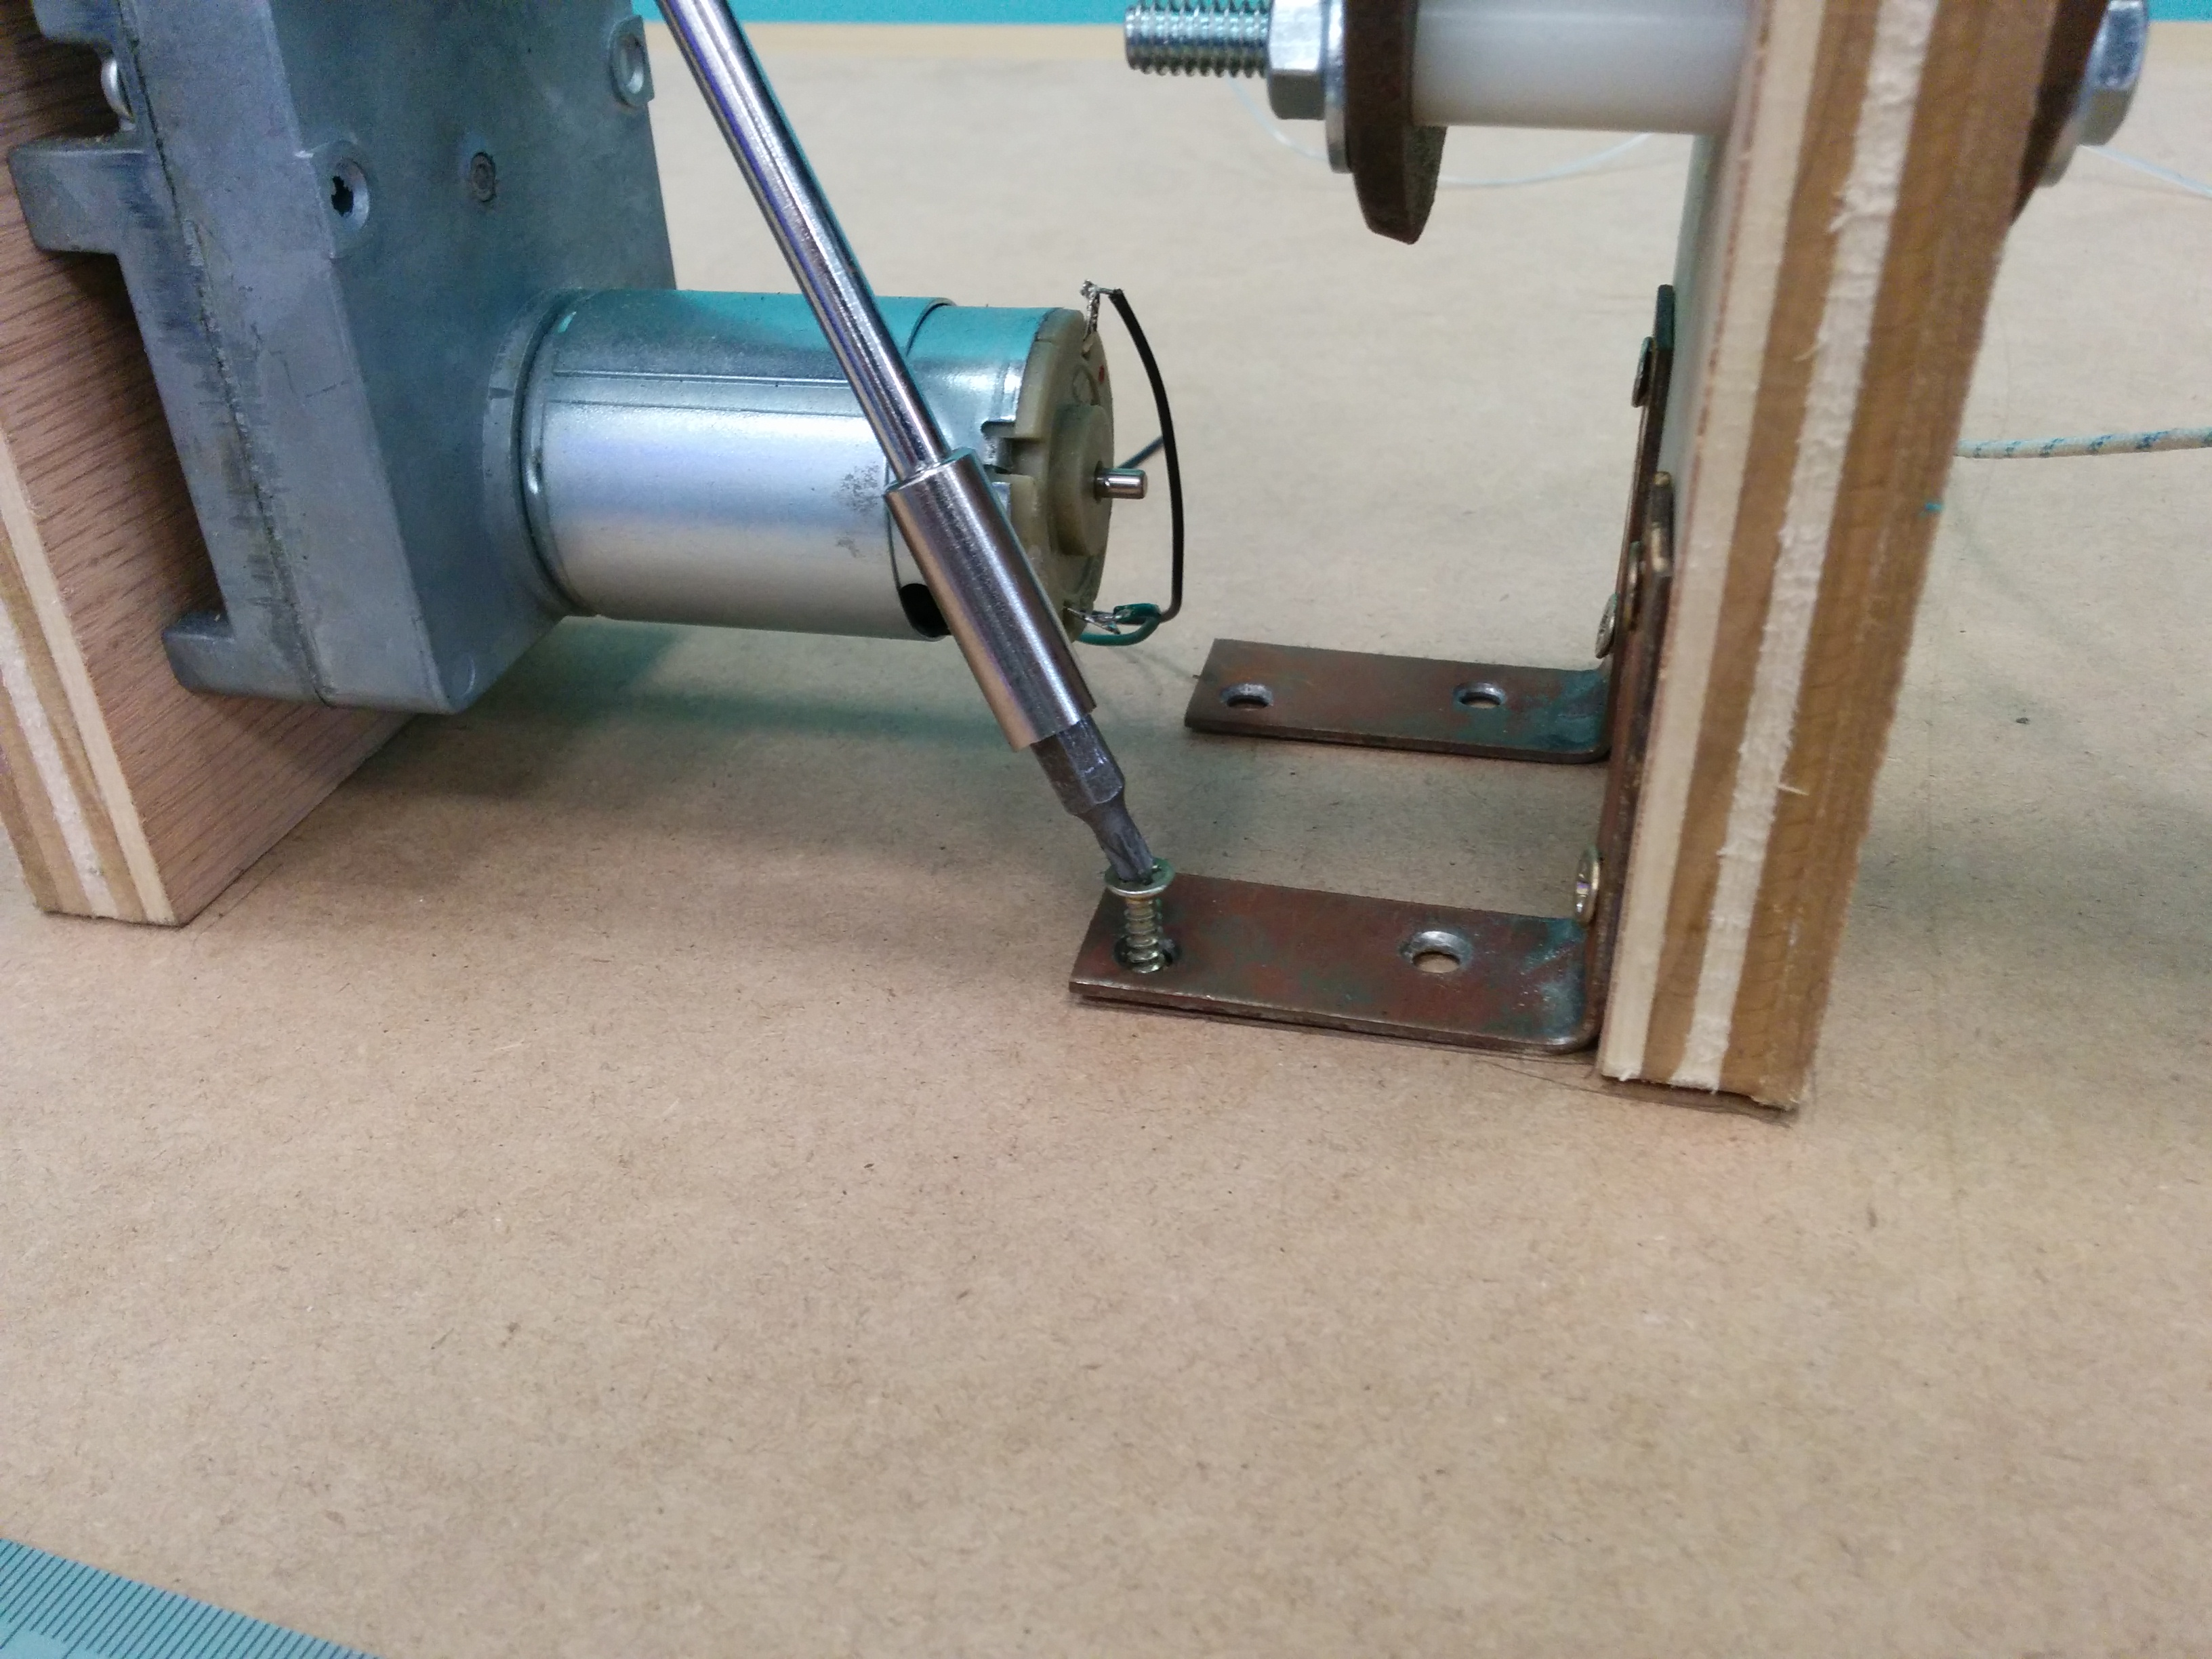
\includegraphics[width=0.6\textwidth]{images/filaextruder/IMG_20150313_114401.jpg}
            \caption{Se ancla la extructura a la base}
            \label{fig:fila_montaje1}
    \end{figure}
    \begin{figure}[H]
            \centering
            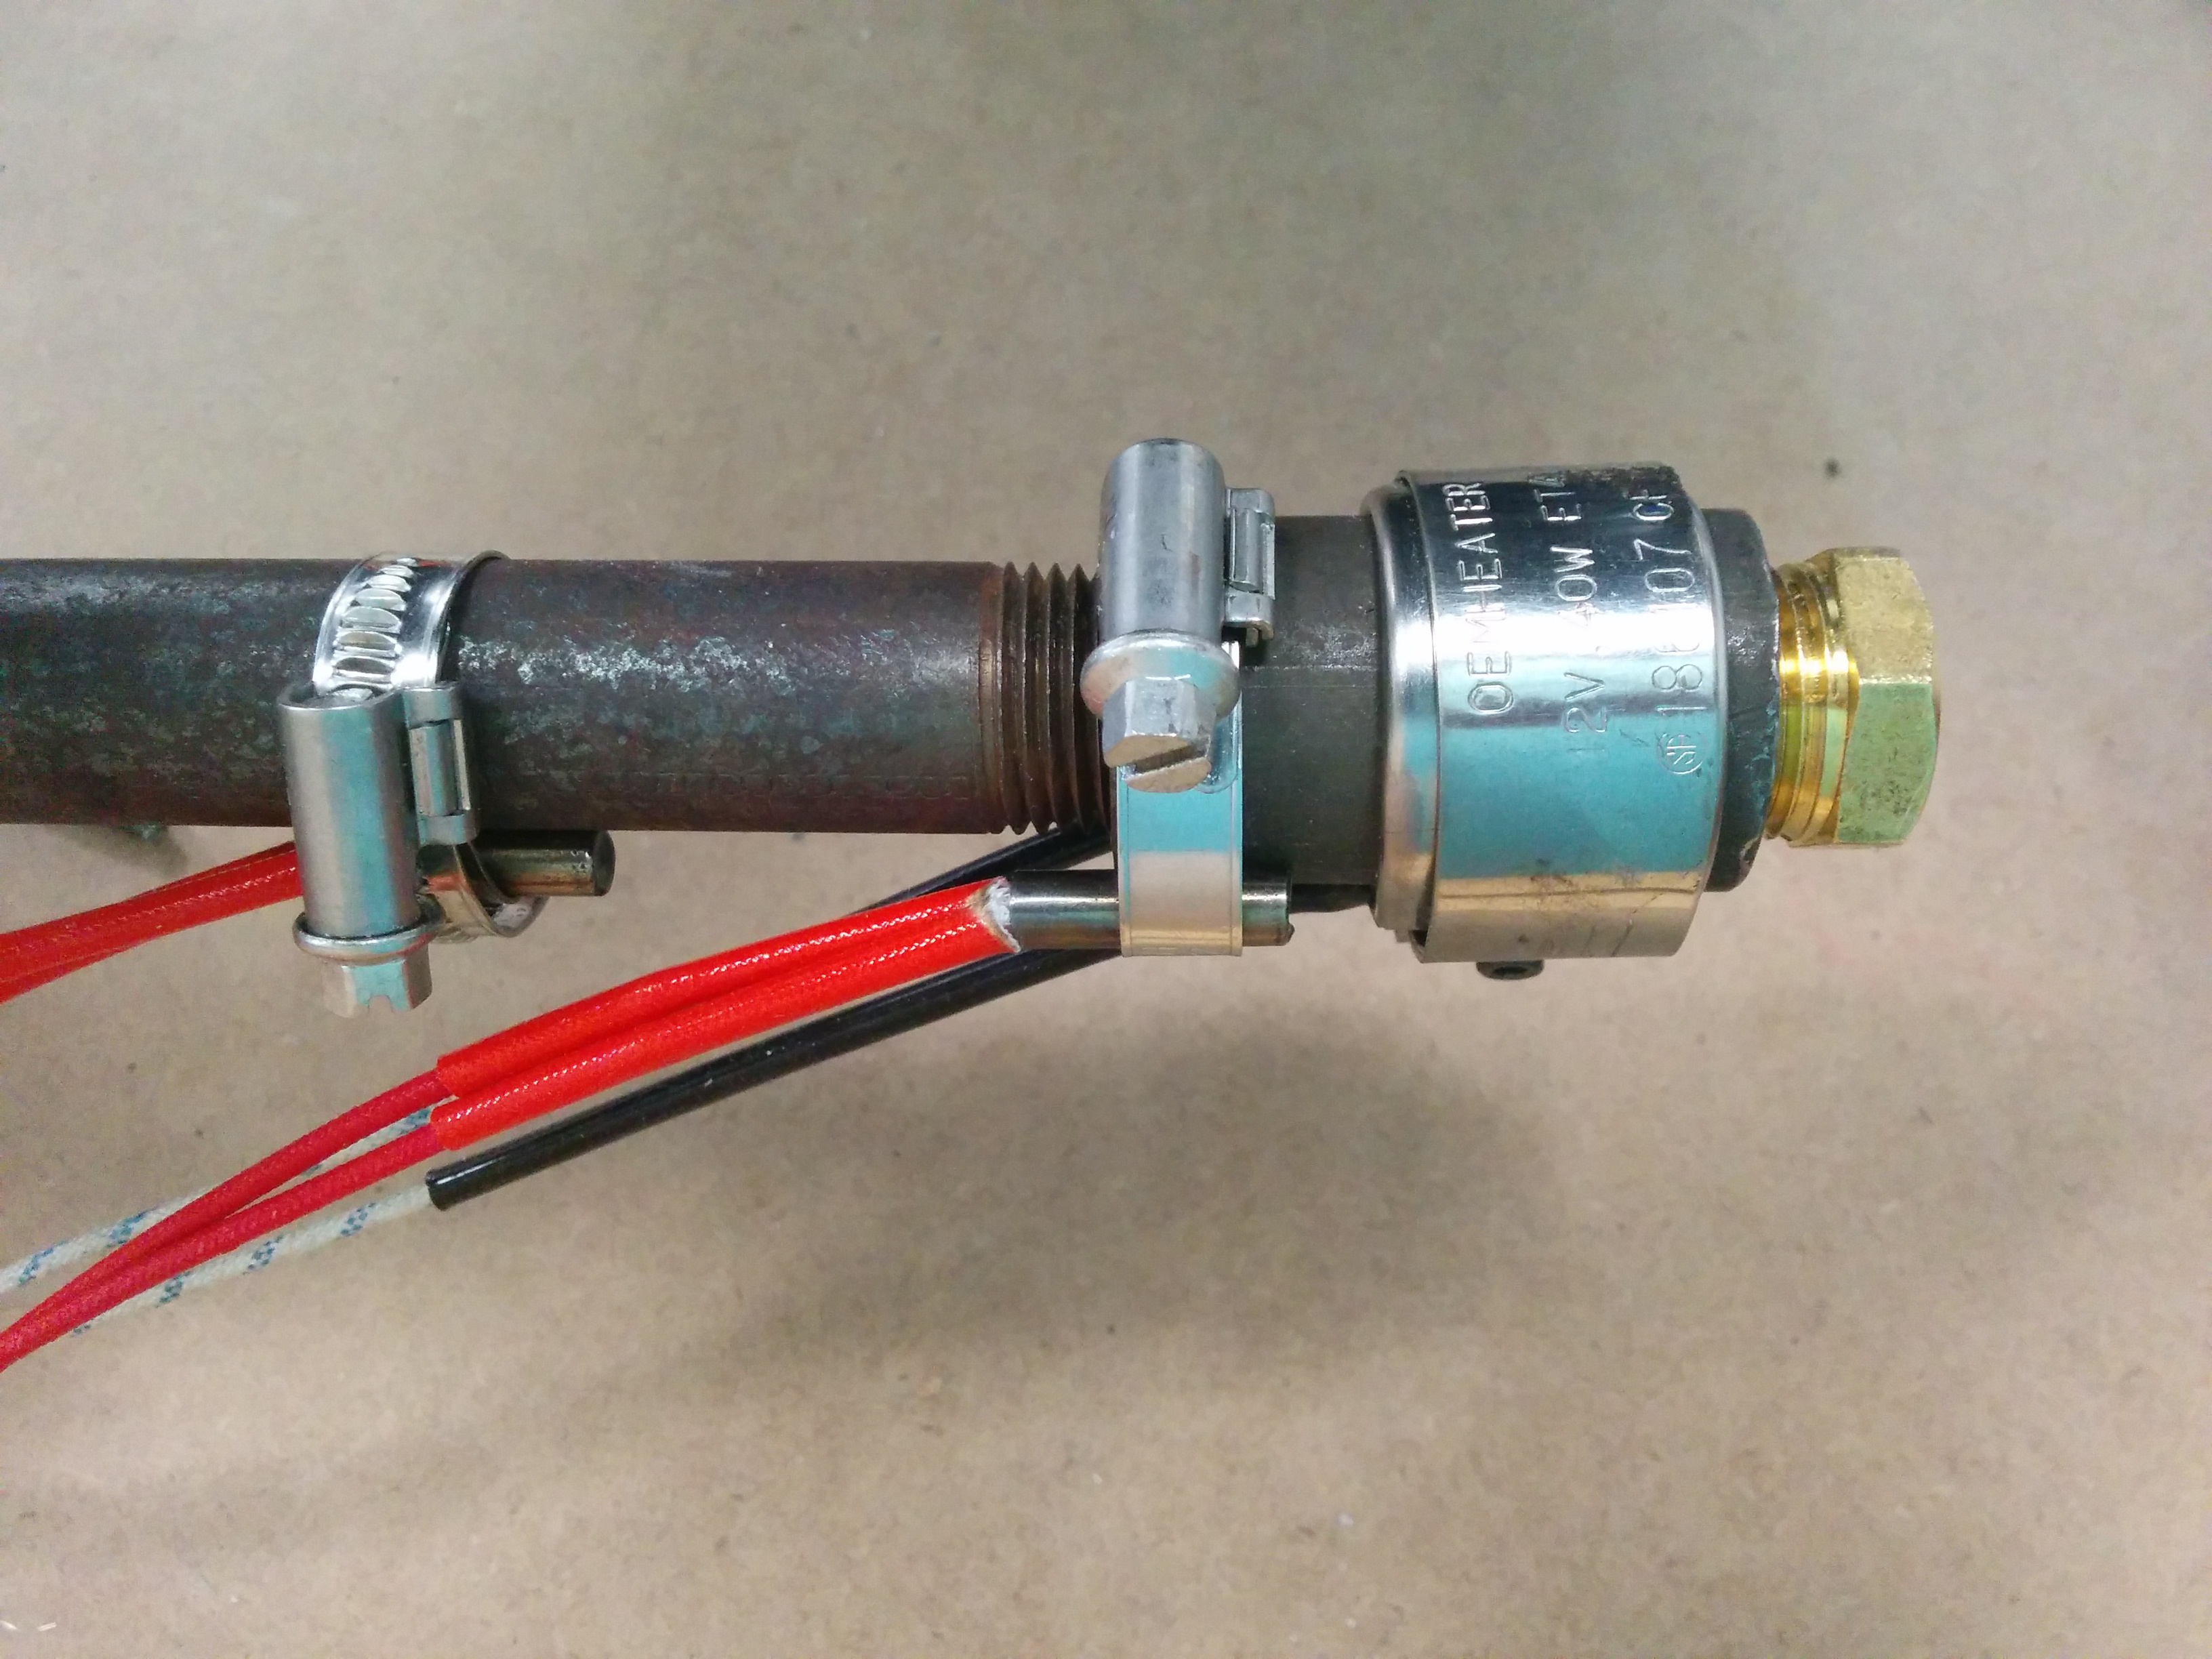
\includegraphics[width=0.6\textwidth]{images/filaextruder/IMG_20150324_175818.jpg}
            \caption{Calefactor en la alimentación y cañon}
            \label{fig:fila_montaje2}
    \end{figure}
    \begin{figure}[H]
            \centering
            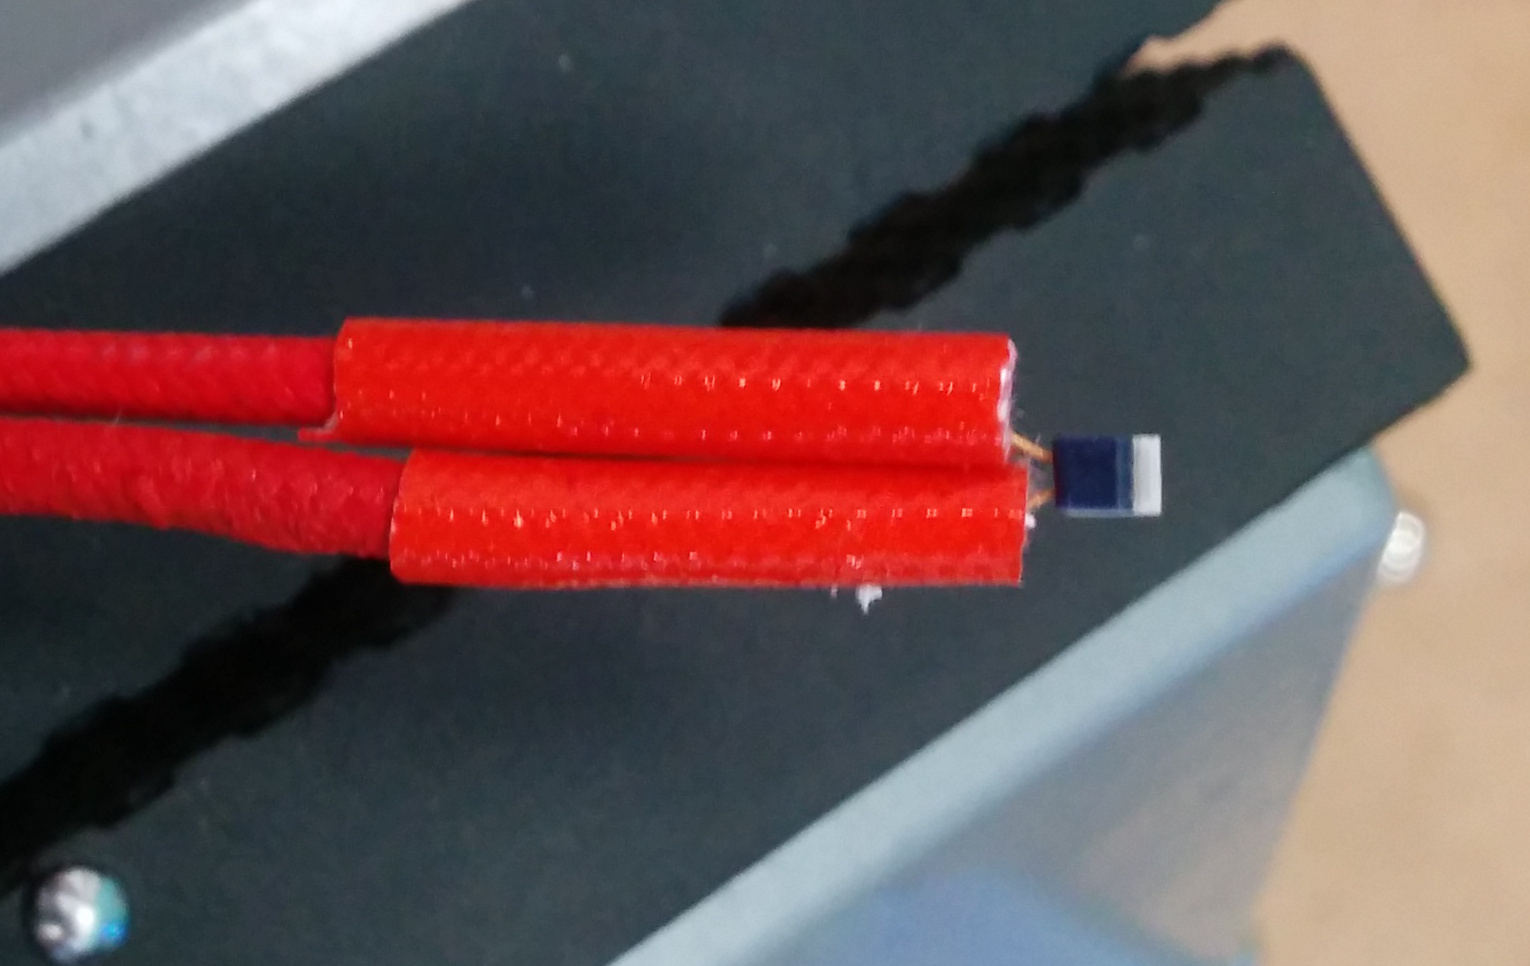
\includegraphics[width=0.6\textwidth]{images/filaextruder/IMG_20150325_145634.jpg}
            \caption{Sensor PT100 de temperatura}
            \label{fig:fila_montaje3}
    \end{figure}

Una vez instalados los cartuchos y las sondas de temperatura en la filastruder, se pasa a aislar el cañón para que la disipación de calor al exterior no sea elevada y poder mantener una temperatura constante.\\

    \begin{figure}[H]
            \centering
            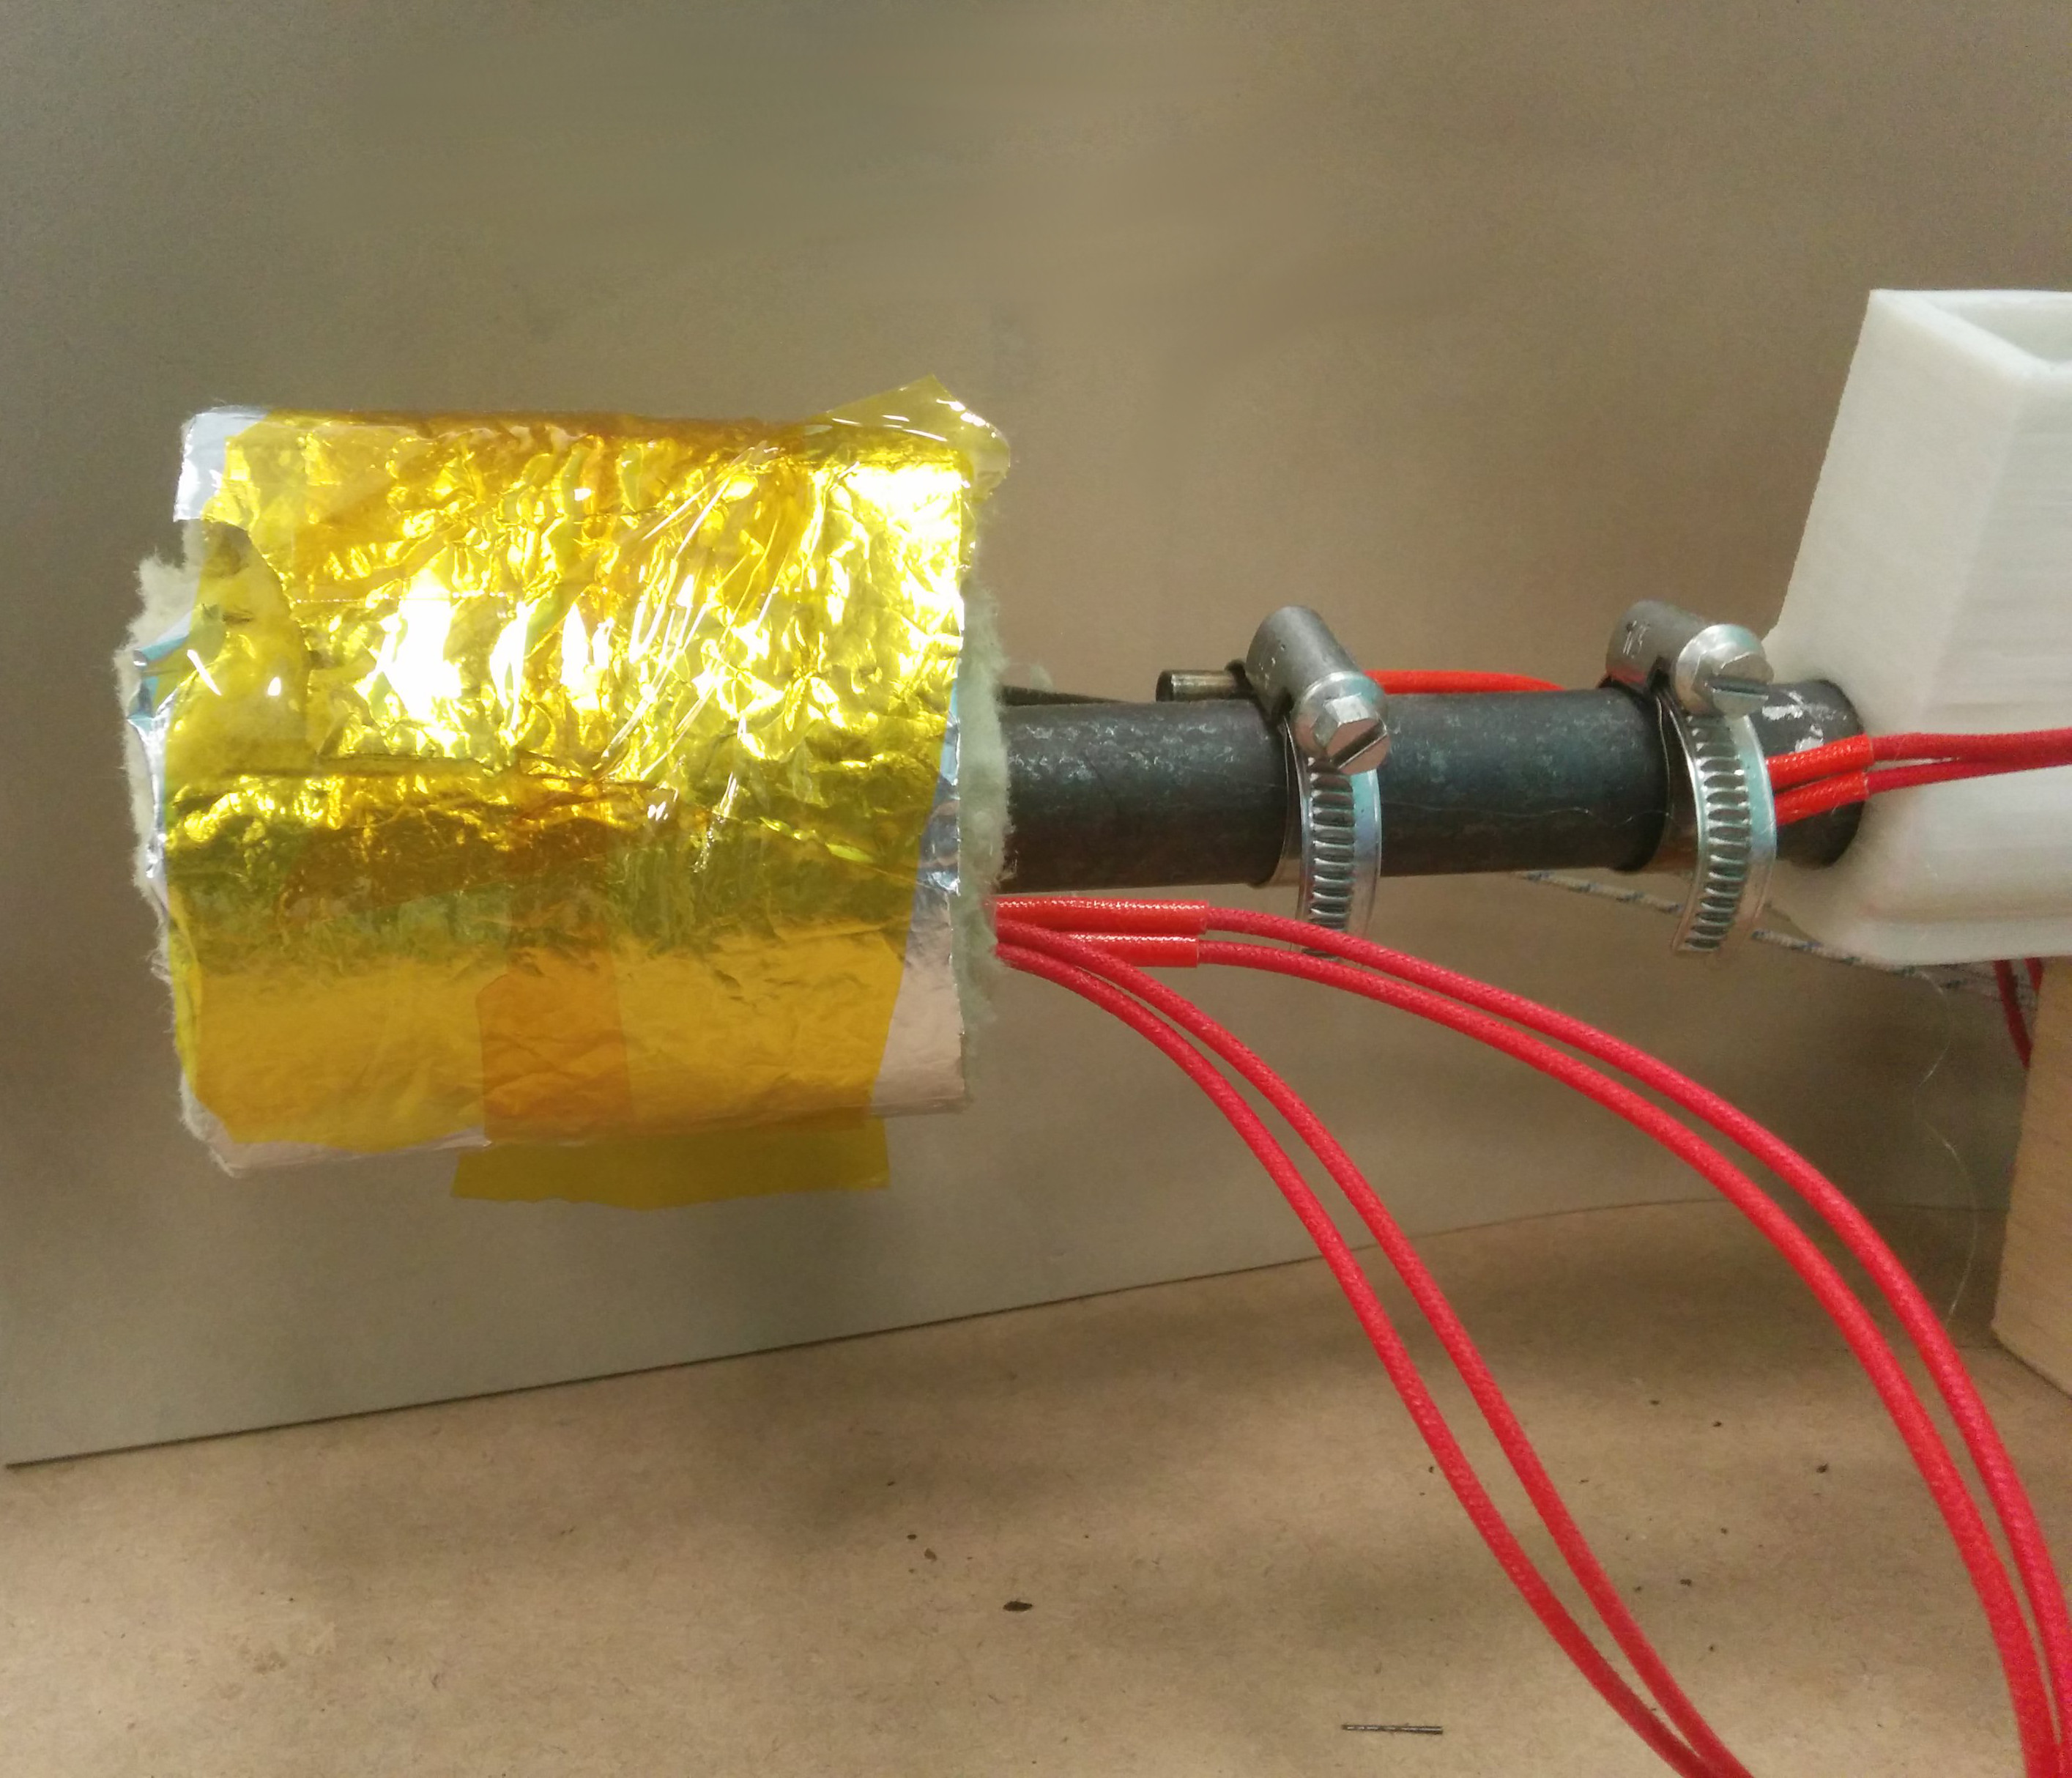
\includegraphics[width=0.4\textwidth]{images/filaextruder/IMG_20150814_132929.jpg}
            \caption{Filastruder montado}
            \label{fig:fila_montaje4}
    \end{figure}

El siguiente paso es cablear todas las señales a un armario que instalaremos en la propia maqueta en el espacio reservado para ello, este armario estará conectado al armario del PLC para poder realizar el control de la maqueta:\\

    \begin{itemize}
    	\item Sondas de temperatura.
    	\item Reles para controlar las resistencias de potencia y el motor del husillo.
    \end{itemize}

El circuito eléctrico a cablear está indicado en el Anexo \ref{ane:esquemas_electricos}.\\

    \begin{figure}[H]
            \centering
            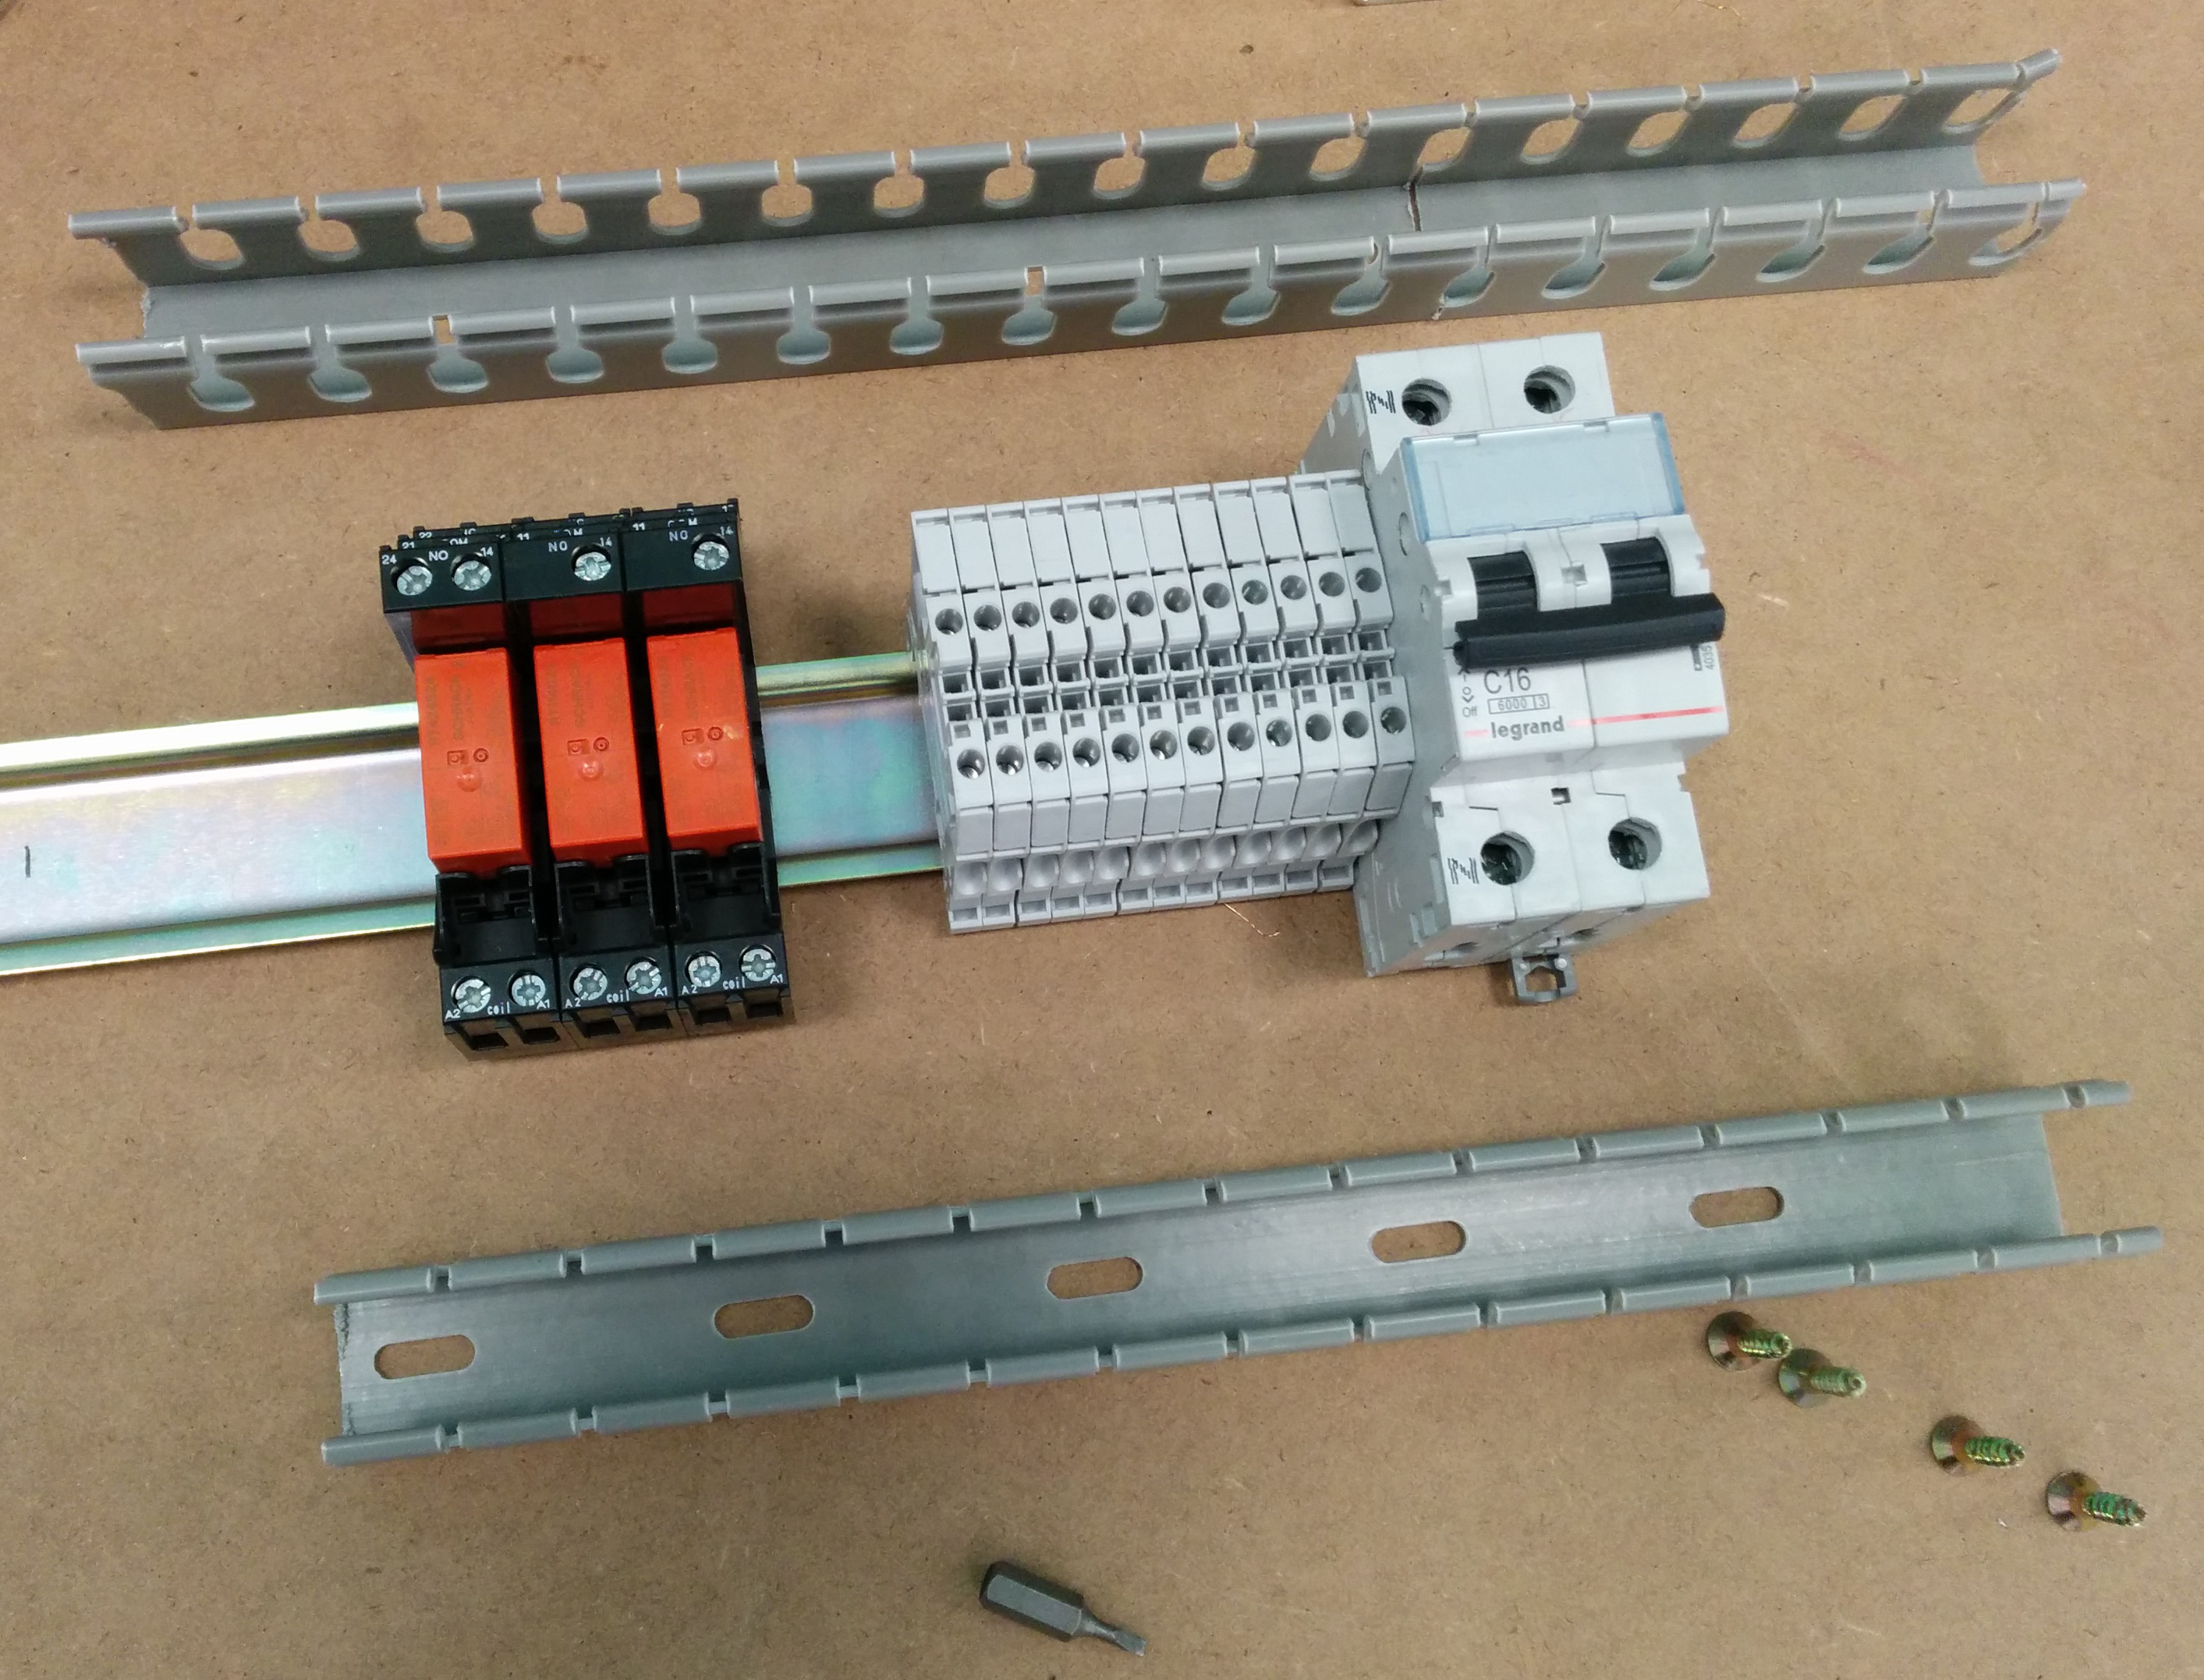
\includegraphics[width=0.5\textwidth]{images/maqueta/IMG_20150324_162200.jpg}
            \caption{Presentación de los componentes en el lugar adecuado.}
            \label{fig:maque_montaje5}
    \end{figure}
    \begin{figure}[H]
            \centering
            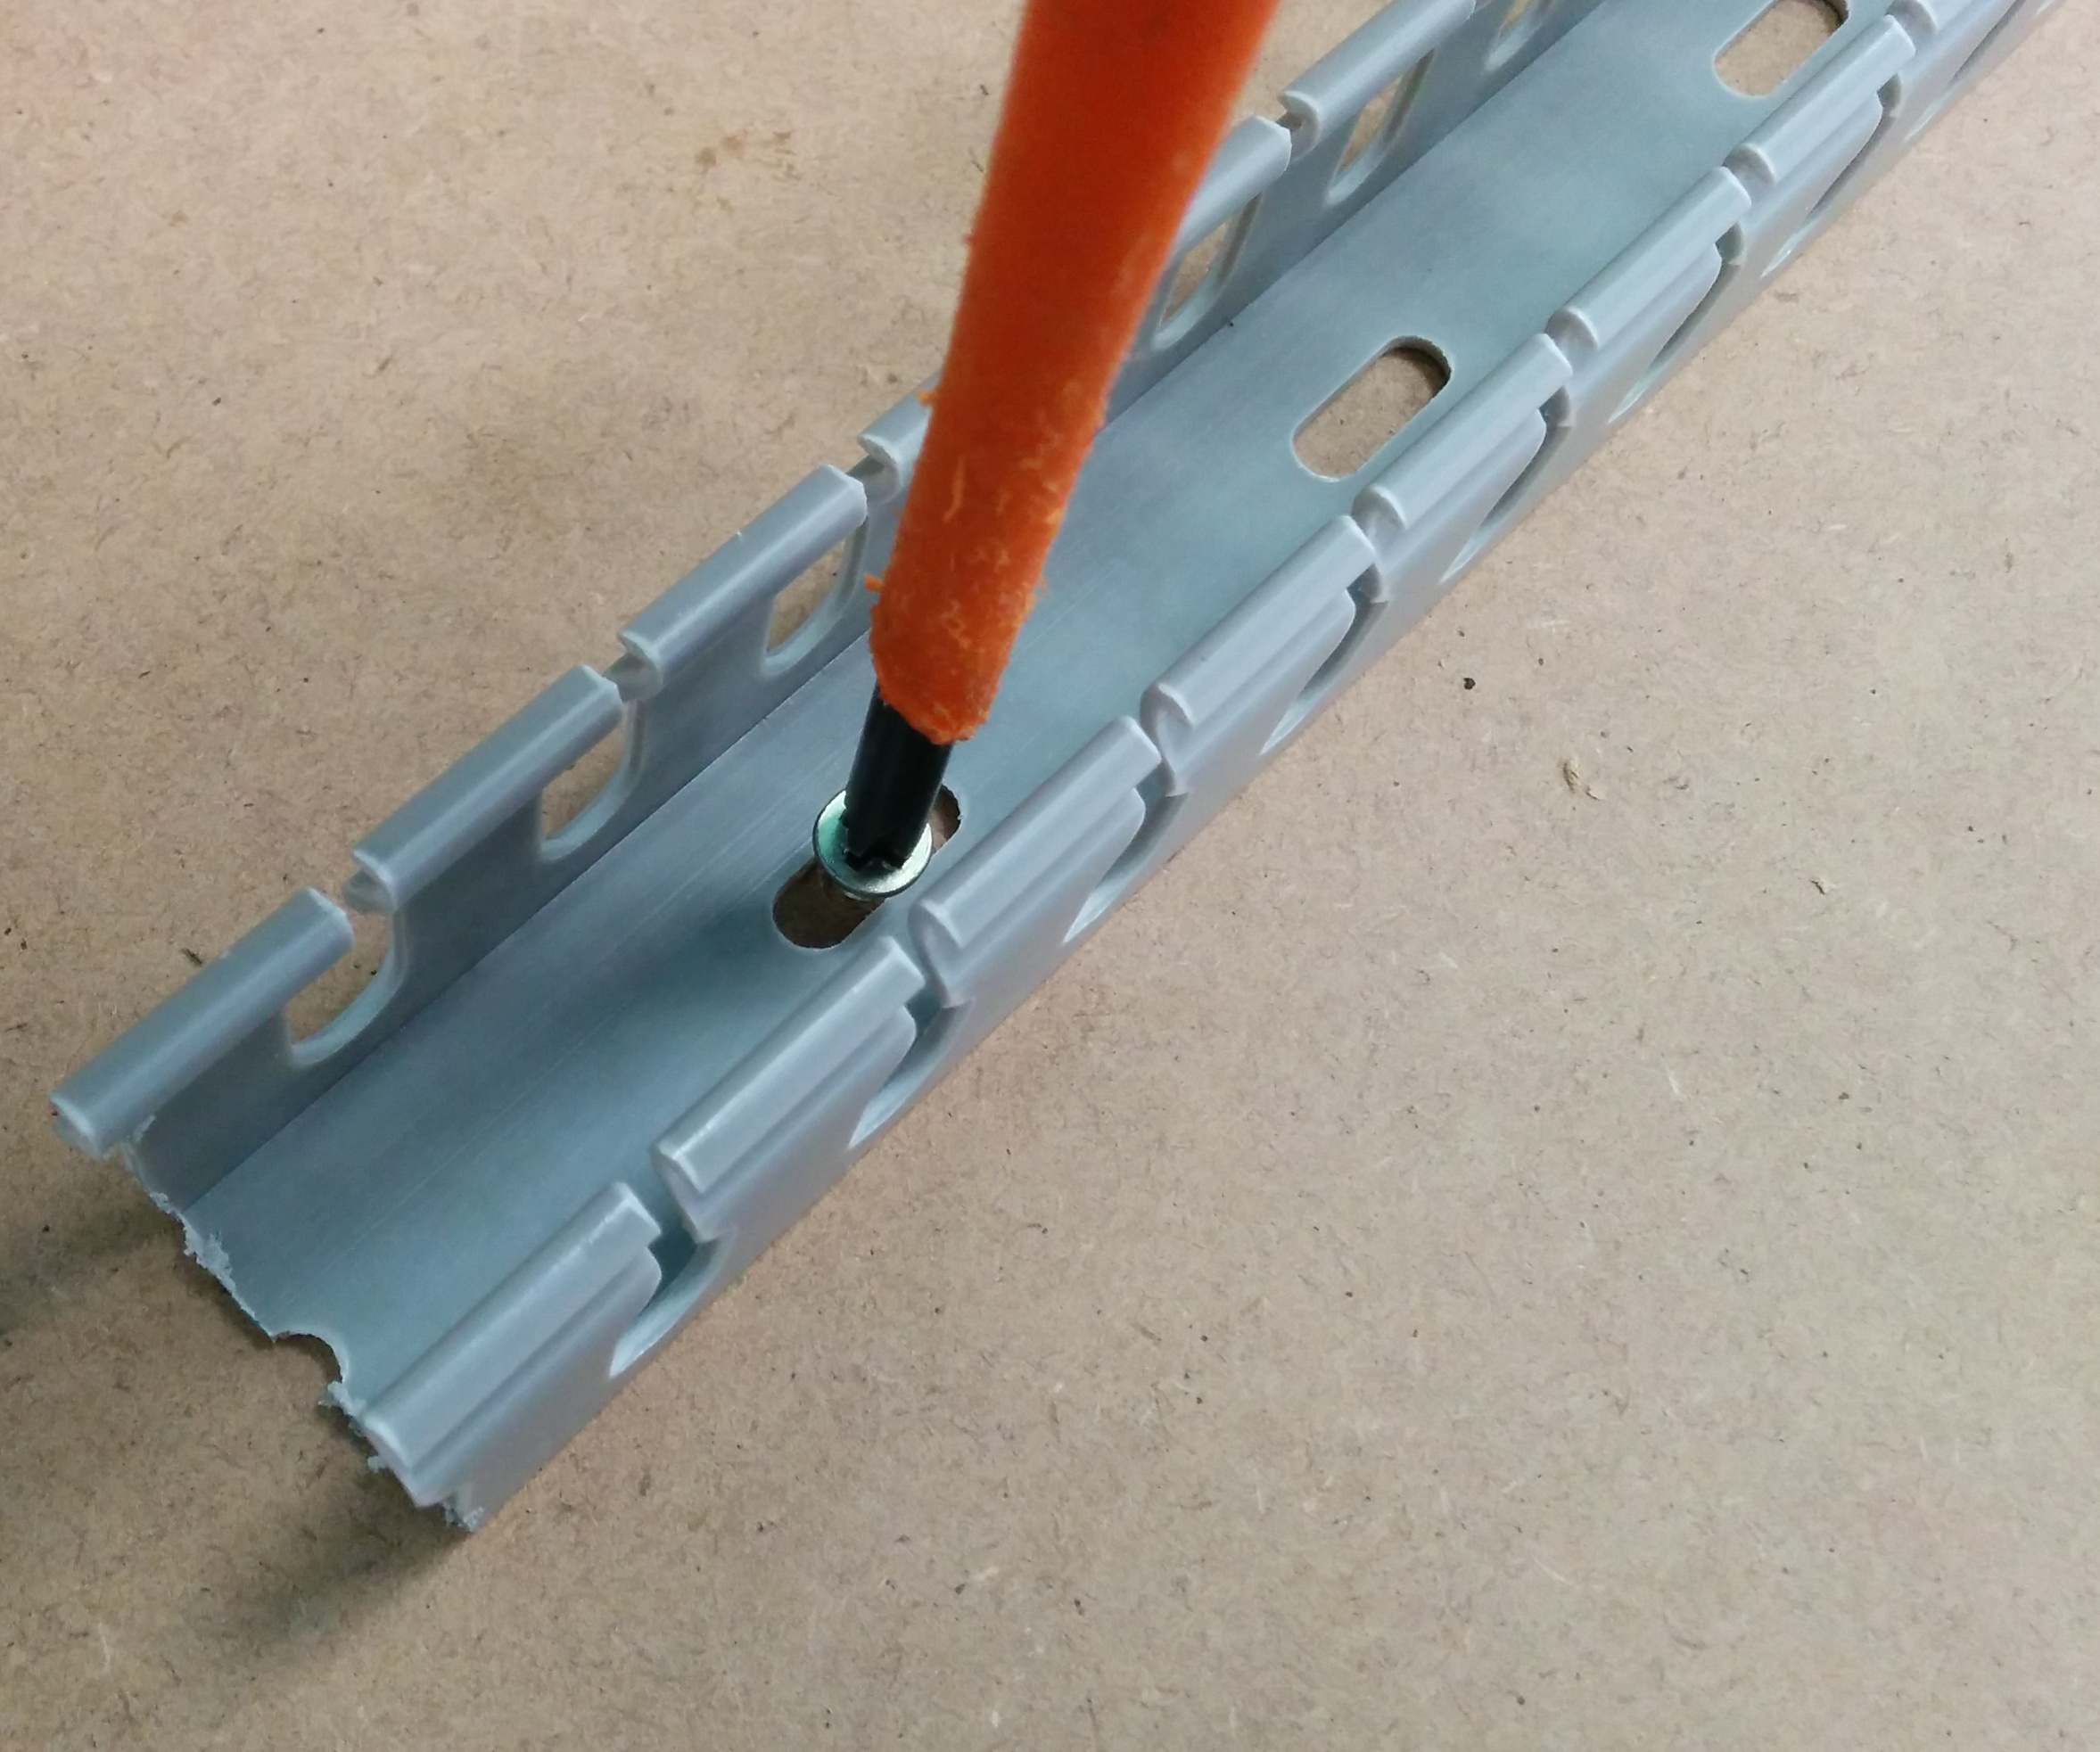
\includegraphics[width=0.5\textwidth]{images/maqueta/IMG_20150324_162705.jpg}
            \caption{Atornillamos las canaletas y guias a la madera.}
            \label{fig:maque_montaje6}
    \end{figure}
    \begin{figure}[H]
            \centering
            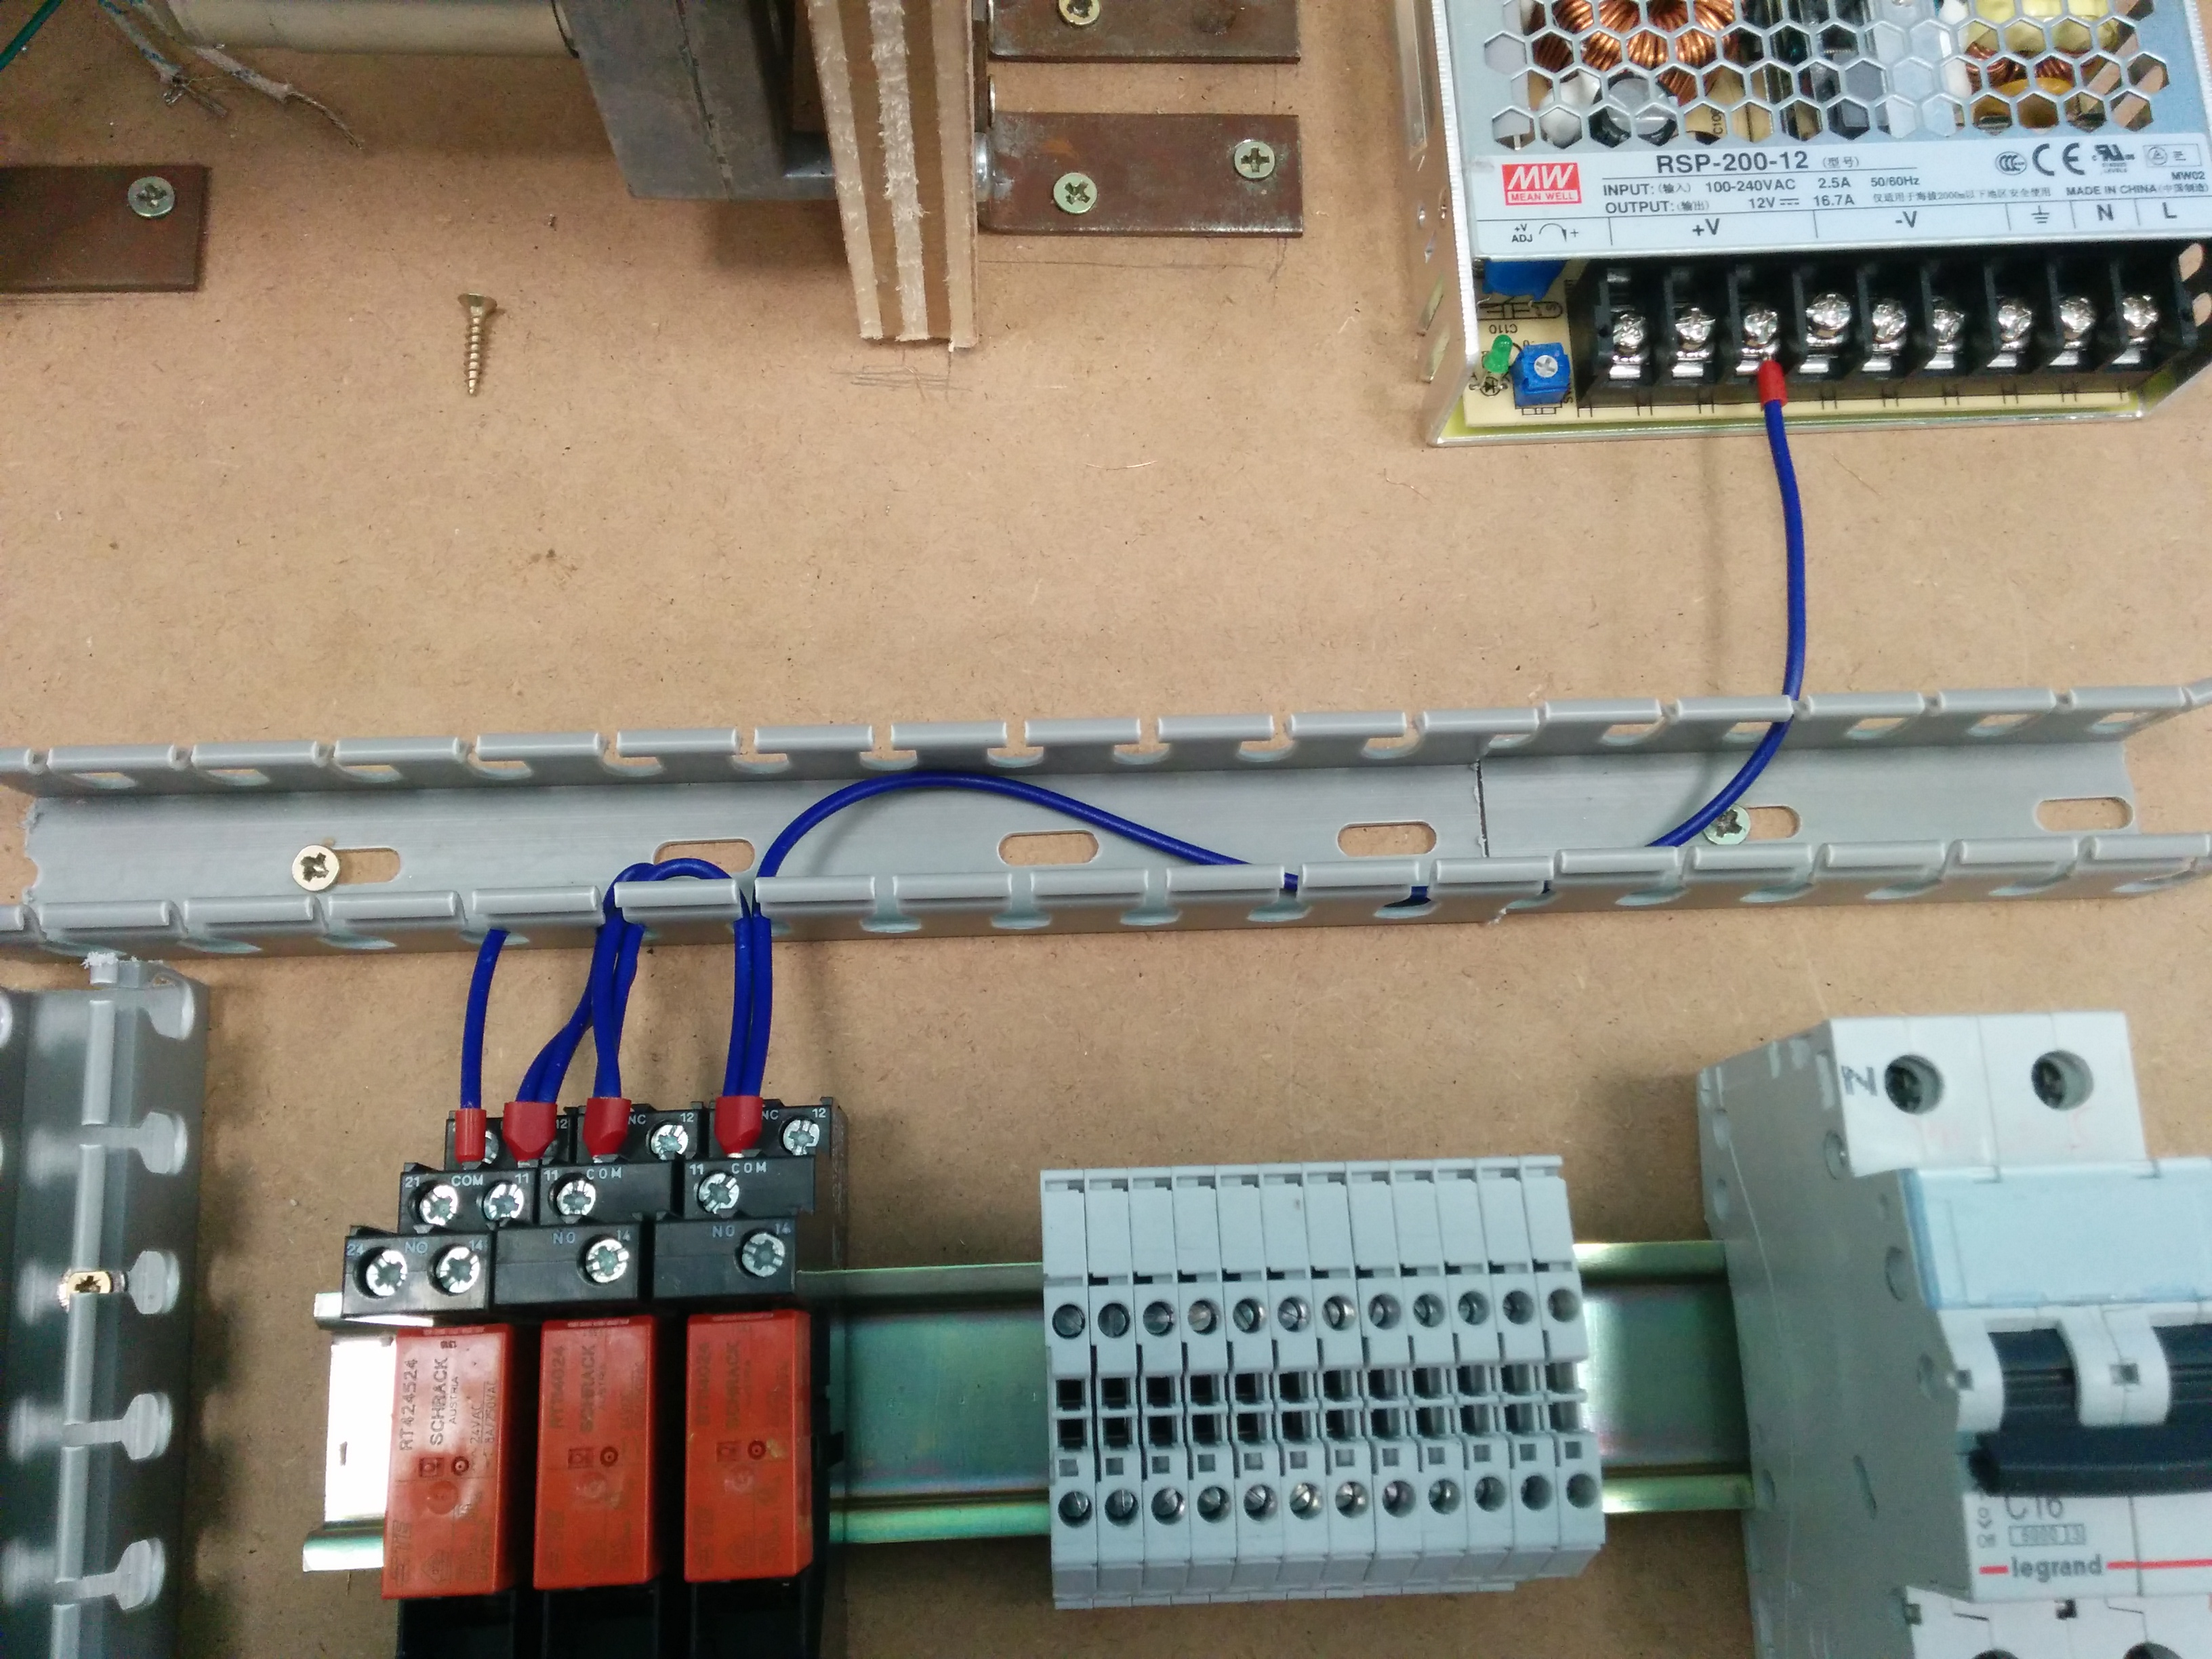
\includegraphics[width=0.5\textwidth]{images/maqueta/IMG_20150324_173716.jpg}
            \caption{Cableamos los componentes según los esquemas.}
            \label{fig:maque_montaje7}
    \end{figure}
    \begin{figure}[H]
            \centering
            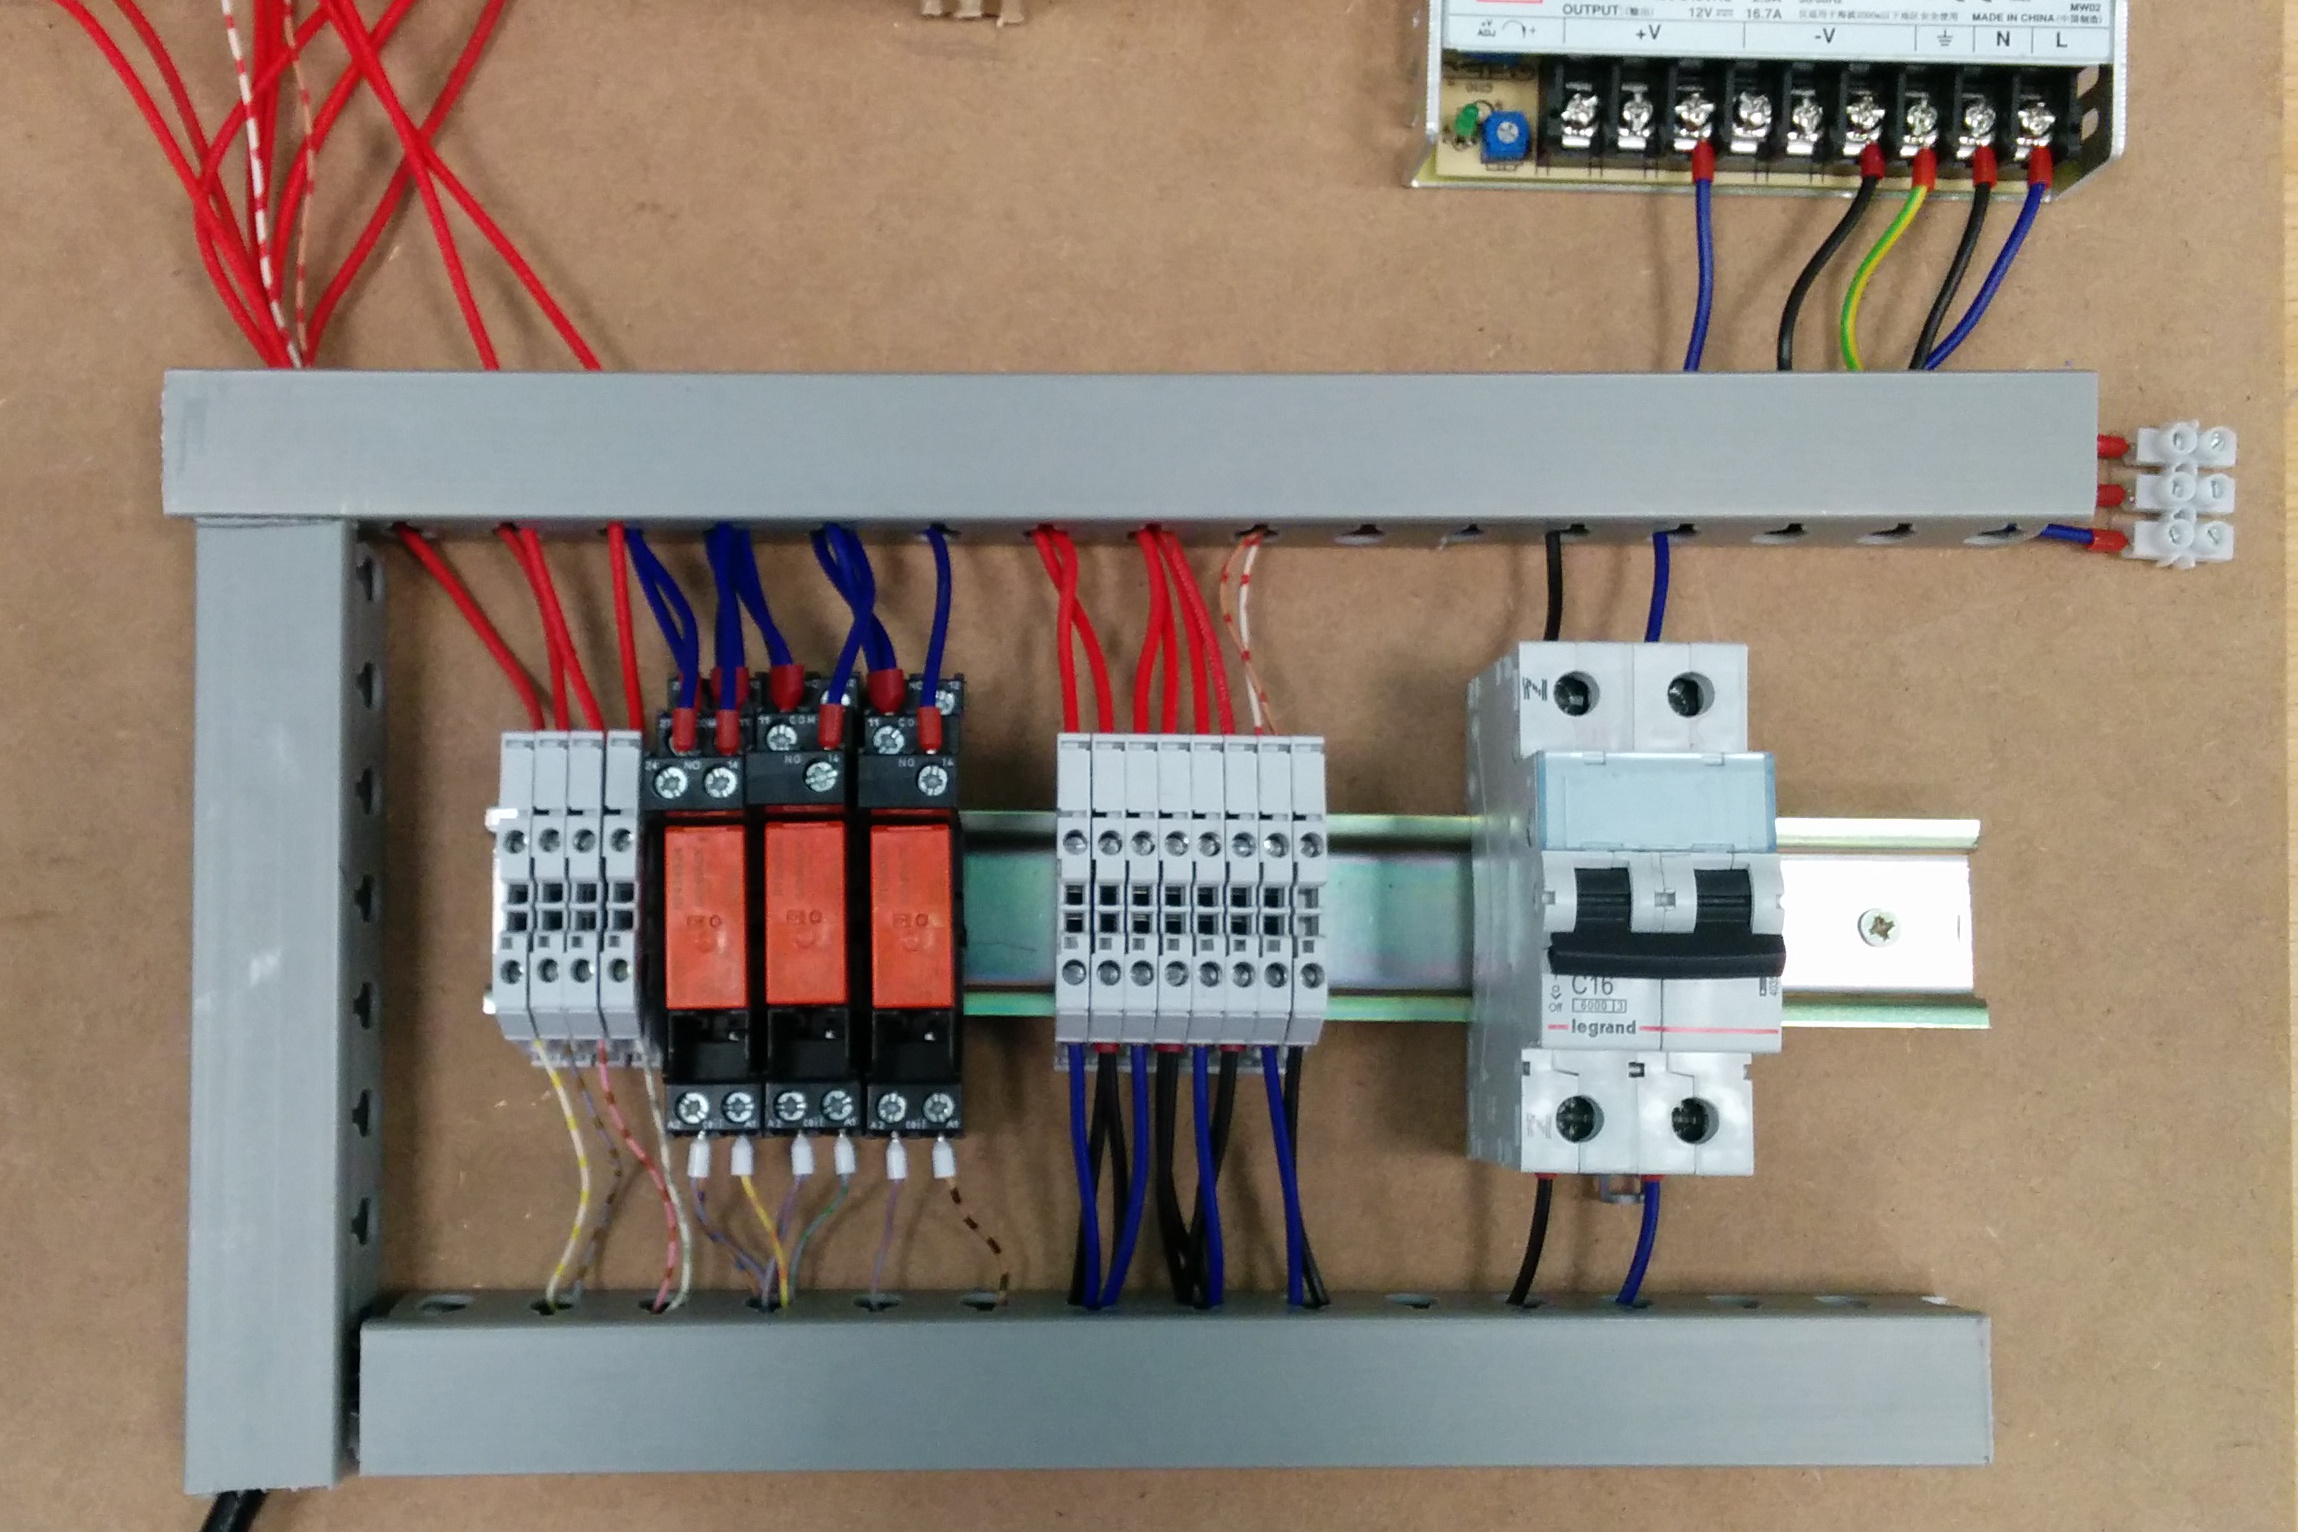
\includegraphics[width=0.5\textwidth]{images/maqueta/IMG_20150331_125243.jpg}
            \caption{Aspecto final cuadro eléctrico maqueta.}
            \label{fig:maque_montaje8}
    \end{figure}